\documentclass[aspectratio=169, 10pt]{beamer}

\usetheme{focus}

% Paleta SupaClock
\definecolor{main}{RGB}{57, 110, 184}
\definecolor{background}{RGB}{255, 255, 255}
\definecolor{accent}{RGB}{63, 185, 80}
\definecolor{warn}{RGB}{218, 54, 51}
\definecolor{softgray}{RGB}{245, 247, 250}

\setbeamercolor{alerted text}{fg=red!80!black}

\usepackage[spanish]{babel}
\usepackage[utf8]{inputenc}
\usepackage[T1]{fontenc}
\usepackage{graphicx}
\usepackage{booktabs}
\usepackage{array}
\usepackage{tikz}
\usepackage{pgfplots}
\pgfplotsset{compat=1.18}
\usetikzlibrary{shapes.geometric, arrows.meta, positioning, fit, backgrounds, calc, babel}

\setbeamerfont{itemize/enumerate body}{size=\small}
\setbeamerfont{itemize/enumerate subbody}{size=\footnotesize}

% Recursos: carpeta actual, assets de Entrega2, renders mecanicos y KiCad.
\graphicspath{{./}{../Entrega2/}{../Entrega2/presentacion_v2/}{../../mechanical/}{../../hardware/SupaClock_Carrier/}}

\title{Wearable ``SupaClock''}
\subtitle{Avance 3 \textbar{} Integraci\'on ESP32-S3, PCB prototipo y carcasa}
\date{\today}
\author{Grupo 10}
\institute{Ingenier\'ia El\'ectrica}
\titlegraphic{\hfill
\includegraphics[height=1.8cm]{logo.pdf}}

\begin{document}

\maketitle

\begin{frame}{Contexto, Requisitos y Soluci\'on}
    \begin{columns}[T]
        \column{0.5\textwidth}
        \footnotesize
        \textbf{Problem\'atica}:
        \begin{itemize}\itemsep0pt
            \item Alta tasa de sedentarismo y sobrepeso en la poblaci\'on.
            \item Necesidad de fomentar h\'abitos saludables mediante monitoreo preventivo y accesible.
        \end{itemize}
        \vspace{0.2cm}
        \textbf{Requisitos de dise\~no}:
        \begin{itemize}\itemsep0pt
            \item \textbf{Factor de forma}: \textit{smartwatch} compacto y aut\'onomo.
            \item \textbf{Biometr\'ia 5-en-1}: SpO\textsubscript{2}, ritmo card\'iaco, temperatura, pod\'ometro y ECG monocanal.
            \item \textbf{Procesamiento edge}: clasificaci\'on local de actividad y telemetr\'ia BLE.
        \end{itemize}
        \column{0.5\textwidth}
        \footnotesize
        \textbf{Soluci\'on propuesta: \textit{SupaClock}}
        \begin{itemize}\itemsep0pt
            \item Wearable de monitoreo continuo con enfoque biom\'etrico y ``cero distracciones''.
            \item \textbf{Hardware}: ESP32, sensores biom\'etricos, IMU y pantalla LCD a color.
            \item \textbf{Ecosistema}: mediciones locales, registro de datos y comunicaci\'on hacia app/gateway.
        \end{itemize}
        \vspace{0.2cm}
        \centering
        
\includegraphics[height=2.7cm]{supaclock_logo.png}
        \vspace{0.05cm}\newline
        \scriptsize\textbf{Figura}: \textit{Identidad visual del proyecto SupaClock.}
    \end{columns}
\end{frame}

\begin{frame}{Objetivo de esta entrega}
    \begin{columns}[T]
        \column{0.55\textwidth}
        \footnotesize
        Esta presentaci\'on consolida los avances posteriores a Entrega 2 y ordena el trabajo hacia el prototipo integrado.
        \vspace{0.25cm}
        \begin{itemize}\itemsep0.16cm
            \item Migraci\'on del banco de desarrollo al \textbf{Seeed XIAO ESP32-S3}.
            \item Cierre del \textbf{dise\~no de PCB carrier} para el prototipo.
            \item Desarrollo de \textbf{carcasa param\'etrica en OpenSCAD}.
            \item Integraci\'on con firmware ya validado: sensores, GUI, BLE, ECG y tareas FreeRTOS.
        \end{itemize}
        \column{0.45\textwidth}
        \centering
        
\includegraphics[width=0.78\linewidth]{supaclock_logo.png}
        \vspace{0.3cm}
        \begin{block}{Foco}
            \scriptsize Pasar de subsistemas validados en protoboard a una unidad wearable ensamblable, repetible y testeable.
        \end{block}
    \end{columns}
\end{frame}

\begin{frame}{Índice}
    \Large
    \centering
    \vspace{0.75cm}
    \begin{enumerate}\itemsep0.35cm
        \item \textbf{Estado de la Entrega 2}
        \item \textbf{Implementaci\'on con XIAO ESP32-S3}
        \item \textbf{PCB final del prototipo}
        \item \textbf{Carcasa param\'etrica en SCAD}
        \item \textbf{Pruebas y siguientes pasos}
    \end{enumerate}
\end{frame}

\section{Estado del Proyecto}

\begin{frame}{Avances consolidados desde Entrega 2}
    \begin{columns}[T]
        \column{0.50\textwidth}
        \scriptsize
        \textbf{Firmware y sensores}
        \begin{itemize}\itemsep0.03cm
            \item FreeRTOS separa ECG, IMU, PPG, GUI, BLE y sistema.
            \item I\textsuperscript{2}C con mutex para BMI160, MAX30102, MAX30205 y MAX17048.
            \item ECG AD8232 por ADC/DMA; Pan-Tompkins validado offline.
            \item LVGL sobre ST7789 con navegaci\'on multipantalla.
            \item Deep sleep, wake-up por IMU, sensores low-power y BLE segmentado.
        \end{itemize}
        \column{0.50\textwidth}
        \scriptsize
        \textbf{Integraci\'on y prototipado}
        \begin{itemize}\itemsep0.03cm
            \item ESP32-C3 valid\'o drivers, pero qued\'o justo en potencia, memoria y margen de ML.
            \item Capacitores externos entregan el pulso inicial de potencia requerido por el ESP32-C3 al encender.
            \item Nueva ESP32-S3 validada en la proto para avanzar hacia el carrier final.
            \item PCB de dos caras: top con display, ECG y botones; bottom con PPG, temperatura y pads ECG.
            \item Carcasa SCAD orientada a fijar PCB, electrodos, sensor \'optico, placa t\'ermica y correa.
        \end{itemize}
    \end{columns}
    \vspace{0.12cm}
    {\scriptsize\textbf{Cambio clave:} la ruta del prototipo final se centra en XIAO ESP32-S3 + carrier propio + carcasa SCAD.}
\end{frame}

\begin{frame}{Arquitectura funcional mantenida}
    \begin{columns}[T]
        \column{0.42\textwidth}
        \scriptsize
        \begin{tabular}{l l}
            \toprule
            \textbf{Bloque} & \textbf{Interfaz} \\
            \midrule
            BMI160 IMU & I\textsuperscript{2}C \\
            MAX30102 PPG/SpO\textsubscript{2} & I\textsuperscript{2}C \\
            MAX30205 temperatura & I\textsuperscript{2}C \\
            MAX17048 fuel gauge & I\textsuperscript{2}C \\
            AD8232 ECG & ADC1 + DMA \\
            ST7789 display & SPI \\
            Botones & GPIO \\
            \bottomrule
        \end{tabular}
        \vspace{0.25cm}
        \begin{itemize}\itemsep0.08cm
            \item Se conserva el particionado por drivers.
            \item El cambio principal es el \textbf{mapa f\'isico de pines} y el soporte mec\'anico.
        \end{itemize}
        \column{0.58\textwidth}
        \vspace{-0.25cm}
        \begin{flushright}
            \resizebox{1.02\linewidth}{!}{\begin{tikzpicture}[
    node distance=0.6cm and 0.9cm,
    every node/.style={font=\scriptsize},
    blockOK/.style={rectangle, rounded corners, draw=black!70, very thick, fill=green!22, text width=3.0cm, align=center, minimum height=0.95cm},
    blockPart/.style={rectangle, rounded corners, draw=black!70, very thick, fill=yellow!28, text width=3.0cm, align=center, minimum height=0.95cm},
    blockTodo/.style={rectangle, rounded corners, draw=black!70, very thick, dashed, fill=red!12, text width=3.0cm, align=center, minimum height=0.95cm},
    pcb/.style={rectangle, rounded corners, draw=blue!70, very thick, fill=blue!10, text width=3.0cm, align=center, minimum height=0.95cm},
    energy/.style={rectangle, rounded corners, draw=black!70, very thick, fill=orange!22, text width=3.0cm, align=center, minimum height=0.9cm},
    mcu/.style={rectangle, rounded corners, draw=black, very thick, fill=blue!22, text width=3.6cm, align=center, minimum height=1.4cm, font=\small\bfseries},
    busI2C/.style={->, >=stealth, thick, blue!70!black},
    busSPI/.style={->, >=stealth, thick, violet!80!black},
    adc/.style={->, >=stealth, thick, orange!85!black},
    gpio/.style={->, >=stealth, thick, teal!70!black},
    ble/.style={->, >=stealth, thick, dashed, blue!60},
    pwr/.style={->, >=stealth, thick, red!70},
    legend/.style={rectangle, draw=black!50, fill=white, inner sep=4pt}
]
% ============== ENERGÍA ==============
\node[energy] (usbc)  {USB-C\\\textit{(prototipo)}};
\node[energy, right=of usbc] (bms)   {BMS TP4056 + DW01A\\\textbf{100\%} (módulo)};
\node[energy, right=of bms]  (lipo)  {Bater\'ia LiPo 3.7\,V\\\textbf{100\%} (502030)};
\node[energy, below=of bms]  (ldo)   {LDO ME6211 3.3\,V\\\textbf{100\%} (módulo)};
\node[blockOK, below=of lipo] (fuel) {MAX17048\\\textbf{100\%} (driver listo)};

% ============== MCU ==============
\node[mcu, right=2cm of fuel] (mcu) {ESP32-C3 SuperMini\\FreeRTOS + LVGL 8.4\\\textbf{Funcionando}};

% ============== SENSORES I2C ==============
\node[blockOK, above=of mcu, xshift=3.3cm] (max205) {MAX30205\\\textbf{100\%} \textit{(0x48)}};
\node[blockOK, right=of max205]            (bmi)    {BMI160 IMU\\\textbf{100\%} \textit{(0x68)}};
\node[blockOK, below=of bmi]               (max102) {MAX30102\\\textbf{95\%} HR/SpO\textsubscript{2}};

% ============== ECG (analógico + DMA) ==============
\node[blockOK, below=of max102] (ad8232) {AD8232 + DMA\\\textbf{90\%} \textit{(GPIO0)}};

% ============== INTERFAZ LOCAL ==============
\node[blockOK, left=2.0cm of mcu] (st7789) {ST7789 1.69" IPS\\\textbf{100\%} (LVGL)};
\node[blockOK, above=of st7789]   (btns)   {3 botones GPIO\\\textbf{100\%} (debounce)};
\node[blockPart, below=of st7789] (gui)    {GUI: Home/Bio/ECG/Menu\\\textbf{85\%} (4 pant.)};

% ============== ECOSISTEMA ==============
\node[blockOK, below=2.4cm of mcu, xshift=-0.4cm] (ble) {BLE NimBLE\\\textbf{100\%} (3 GATT chr.)};
\node[blockPart, right=of ble]                     (cli) {Cliente PC testing\\\textbf{60\%} (\texttt{ble\_logger.py})};
\node[blockOK, right=of cli]                       (fb)  {Firebase + Pan-Tompkins\\\textbf{100\%} (Cloud Fn)};
\node[blockTodo, below=of fb]                      (ml)  {TinyML (CNN 1D)\\\textbf{0\%} (rec.\ datos)};
\node[blockTodo, below=of cli]                     (pcb) {PCB SuperMini propia\\\textbf{30\%} (KiCad WIP)};
\node[blockTodo, below=of ble]                     (app) {App m\'ovil (gateway)\\\textbf{0\%} (hito 60\%)};

% ============== Conexiones de potencia ==============
\draw[pwr] (usbc)  -- (bms);
\draw[pwr] (bms)   -- (lipo);
\draw[pwr] (bms)   -- (ldo);
\draw[pwr] (lipo)  -- (fuel);
\draw[pwr] (ldo.east)  -- ++(0.3,0) |- (mcu.west);

% ============== Buses I2C ==============
\draw[busI2C] (max205) -- node[above]{I2C 400\,kHz} (mcu);
\draw[busI2C] (bmi)    -- (mcu);
\draw[busI2C] (max102) -- (mcu);
\draw[busI2C] (fuel)   -- (mcu);

% ============== ECG analógico ==============
\draw[adc] (ad8232) -- node[below, sloped]{ADC1 / DMA 20\,kHz} (mcu);

% ============== SPI display + GPIO botones ==============
\draw[busSPI] (mcu.west) -- node[above]{SPI 80\,MHz} (st7789.east);
\draw[gpio]   (btns)   -- (mcu.north west);

% ============== BLE / cloud ==============
\draw[ble] (mcu)  -- (ble);
\draw[ble] (ble)  -- node[above]{GATT 3 chr.} (cli);
\draw[gpio, ->] (cli) -- node[above]{Wi-Fi/REST} (fb);
\draw[ble, ->, dashed, gray!60] (ble) -- node[left]{futuro} (app);
\draw[ble, ->, dashed, gray!60] (app) -| (fb);

% ============== Leyenda ==============
\node[legend, below=1.6cm of ble, xshift=4cm] (leg) {%
\begin{tabular}{ll}
\textcolor{green!50!black}{$\blacksquare$} Funcionando &
\textcolor{orange!80!black}{$\blacksquare$} Parcial \\
\textcolor{red!70!black}{$\blacksquare$} Pendiente / dependiente &
\textcolor{red!70}{\textbf{$\rightarrow$}} Potencia \\
\textcolor{blue!70!black}{$\rightarrow$} I2C 400\,kHz &
\textcolor{violet!80!black}{$\rightarrow$} SPI 80\,MHz \\
\textcolor{orange!85!black}{$\rightarrow$} ADC/DMA &
\textcolor{blue!60}{$\dashrightarrow$} BLE / Wi-Fi \\
\end{tabular}};
\end{tikzpicture}
}
            \vspace{0.05cm}\newline
            \scriptsize\textbf{Figura}: Bloques de hardware heredados del informe de avance.
        \end{flushright}
    \end{columns}
\end{frame}

\section{XIAO ESP32-S3}

\begin{frame}{Implementaci\'on sobre Seeed XIAO ESP32-S3}
    \begin{columns}[T]
        \column{0.52\textwidth}
        \footnotesize
        \textbf{Motivaci\'on}
        \begin{itemize}\itemsep0.12cm
            \item Mayor margen de c\'omputo para ML local e inferencia TinyML.
            \item Mejor margen de memoria frente a LVGL, NimBLE, buffers DMA y tareas FreeRTOS.
            \item Plataforma m\'as cercana al prototipo final, con USB-C integrado.
            \item Permite ordenar el dise\~no alrededor de un m\'odulo compacto y reemplazable.
        \end{itemize}
        \vspace{0.15cm}
        \begin{block}{Decisi\'on de dise\~no}
            \scriptsize La v1 del carrier usa XIAO S3 en formato DIP/socket para facilitar reemplazo y debug; versiones posteriores pueden migrar a castellated/SMD.
        \end{block}
        \column{0.48\textwidth}
        \scriptsize
        \textbf{Asignaci\'on principal de pines}
        \vspace{0.1cm}

        \begin{tabular}{l l}
            \toprule
            \textbf{Funci\'on} & \textbf{GPIO XIAO S3} \\
            \midrule
            ECG OUT & GPIO1 / ADC1\_CH0 \\
            ECG SDN & GPIO2 \\
            Backlight PWM & GPIO3 \\
            SPI DC & GPIO4 \\
            I2C SDA/SCL & GPIO5 / GPIO6 \\
            BTN NEXT & GPIO43 \\
            SPI CS & GPIO44 \\
            SPI SCK/MOSI & GPIO7 / GPIO9 \\
            BTN SELECT & GPIO8 \\
            \bottomrule
        \end{tabular}
        \vspace{0.2cm}
        \scriptsize Fuente del proyecto: \texttt{include/supaclock\_pinmap.h}.
    \end{columns}
\end{frame}

\begin{frame}{Bring-up esperado del XIAO S3}
    \begin{columns}[T]
        \column{0.50\textwidth}
        \footnotesize
        \textbf{Ruta de validaci\'on}
        \begin{enumerate}\itemsep0.12cm
            \item Compilar firmware base con target ESP32-S3.
            \item Validar I\textsuperscript{2}C: BMI160, MAX30102, MAX30205, MAX17048.
            \item Validar SPI: ST7789 + LVGL + backlight PWM.
            \item Validar ADC/DMA: AD8232 y captura ECG.
            \item Activar BLE y comprobar telemetr\'ia.
            \item Medir consumo real con el carrier ensamblado.
        \end{enumerate}
        \column{0.50\textwidth}
        \footnotesize
        \textbf{Riesgos tratados desde dise\~no}
        \begin{itemize}\itemsep0.12cm
            \item GPIO43/44 quedan usados por bot\'on y chip-select, por lo que la consola debe ir por USB-Serial-JTAG.
            \item BMI160 INT1 no queda cableado en carrier v1; HAR y podometr\'ia operan por polling/FIFO.
            \item El carrier deja VBUS sin conectar: alimentaci\'on y carga quedan centralizadas en el XIAO.
        \end{itemize}
        \vspace{0.15cm}
        \begin{alertblock}{Criterio}
            \scriptsize No se cambia la arquitectura de firmware hasta comprobar equivalencia funcional con el prototipo C3.
        \end{alertblock}
    \end{columns}
\end{frame}

\section{PCB Final}

\begin{frame}{Dise\~no final de PCB para prototipo}
    \begin{columns}[T]
        \column{0.48\textwidth}
        \footnotesize
        \textbf{Carrier SupaClock v1}
        \begin{itemize}\itemsep0.12cm
            \item PCB propia para integrar el XIAO ESP32-S3 con display, sensores, ECG y botones.
            \item Dise\~no orientado a fabricaci\'on local/laboratorio: 2 capas, reglas LPKF y componentes manejables.
            \item Proyecto KiCad separado en \texttt{hardware/SupaClock\_Carrier}.
            \item Mapa de pines congelado y sincronizado con firmware.
        \end{itemize}
        \vspace{0.15cm}
        \begin{block}{Avance}
            \scriptsize El carrier pasa a ser la fuente f\'isica de integraci\'on: ya no se depende del protoboard para posicionamiento ni cableado.
        \end{block}
        \column{0.52\textwidth}
        \centering
        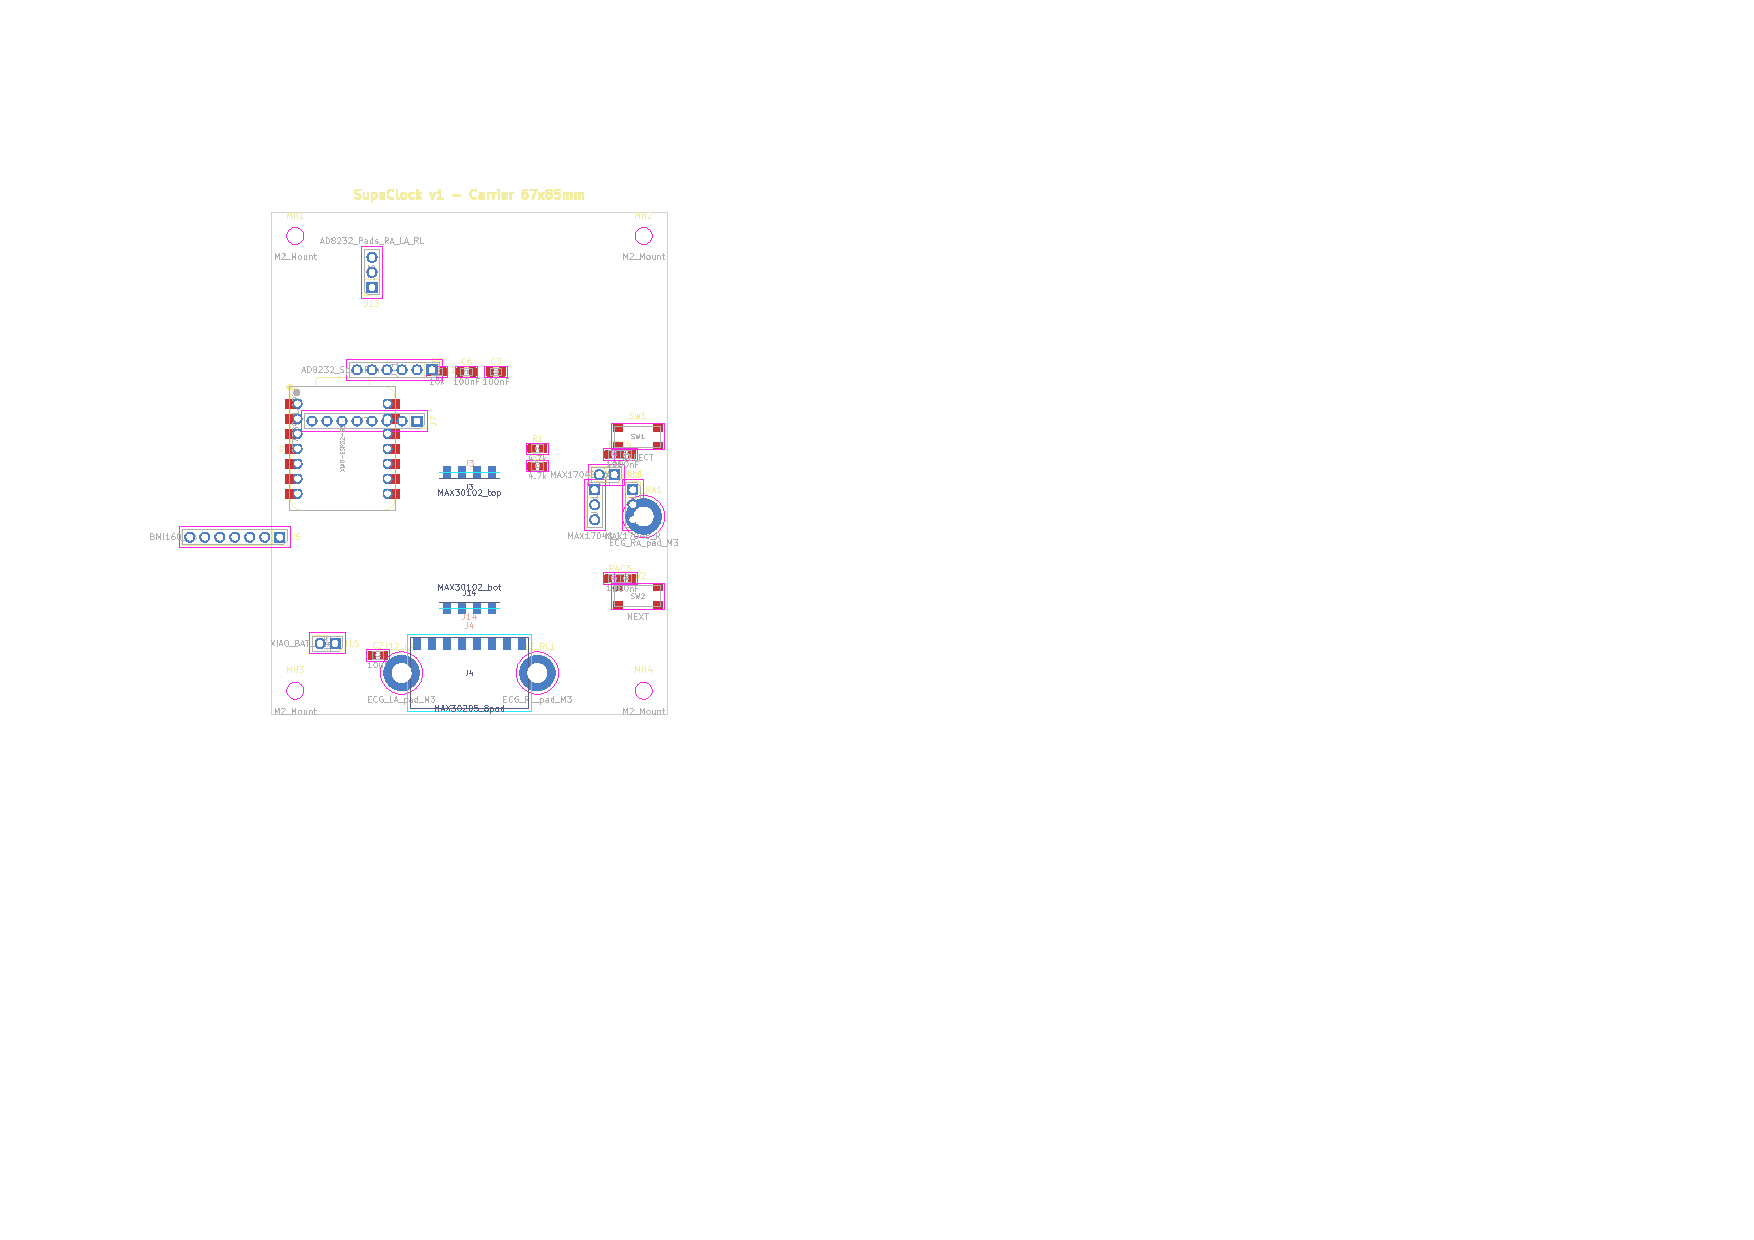
\includegraphics[page=1,width=0.95\linewidth]{SupaClock_Carrier_v1_pcb_placement.pdf}
        \vspace{0.05cm}\newline
        \scriptsize\textbf{Figura}: Placement de la PCB carrier v1.
    \end{columns}
\end{frame}

\begin{frame}{Arquitectura f\'isica de la PCB}
    \begin{columns}[T]
        \column{0.50\textwidth}
        \footnotesize
        \textbf{Cara superior}
        \begin{itemize}\itemsep0.08cm
            \item XIAO ESP32-S3 en socket/header.
            \item Display ST7789 1.69''.
            \item AD8232 para ECG.
            \item MAX17048 como fuel gauge.
            \item Botones laterales y conectores de debug.
        \end{itemize}
        \vspace{0.25cm}
        \textbf{Cara inferior}
        \begin{itemize}\itemsep0.08cm
            \item MAX30102 orientado a piel con ventana \'optica.
            \item MAX30205 acoplado a placa t\'ermica.
            \item Pads de ECG para contacto mediante pogo pins.
        \end{itemize}
        \column{0.50\textwidth}
        \footnotesize
        \begin{block}{Por qu\'e una sola PCB}
            \scriptsize Reduce cableado, mejora repetibilidad mec\'anica y permite alinear sensores, display, botones y carcasa desde el mismo sistema de coordenadas.
        \end{block}
        \vspace{0.2cm}
        \begin{tikzpicture}[
            block/.style={draw=main, rounded corners=2pt, fill=main!8, align=center, minimum width=2.65cm, minimum height=0.65cm, font=\scriptsize},
            arr/.style={->, thick, main}
        ]
            \node[block] (s3) {XIAO ESP32-S3};
            \node[block, below=0.35cm of s3] (pcb) {Carrier PCB v1};
            \node[block, below left=0.45cm and -0.05cm of pcb] (top) {Top: display\\ECG\\botones};
            \node[block, below right=0.45cm and -0.05cm of pcb] (bottom) {Bottom: PPG\\temp\\ECG pads};
            \node[block, below=1.25cm of pcb, fill=accent!10, draw=accent] (case) {Carcasa SCAD\\alineaci\'on mec\'anica};
            \draw[arr] (s3) -- (pcb);
            \draw[arr] (pcb) -- (top);
            \draw[arr] (pcb) -- (bottom);
            \draw[arr] (top) -- (case);
            \draw[arr] (bottom) -- (case);
        \end{tikzpicture}
    \end{columns}
\end{frame}

\begin{frame}{Evoluci\'on respecto al prototipo anterior}
    \begin{columns}[T]
        \column{0.50\textwidth}
        \centering
        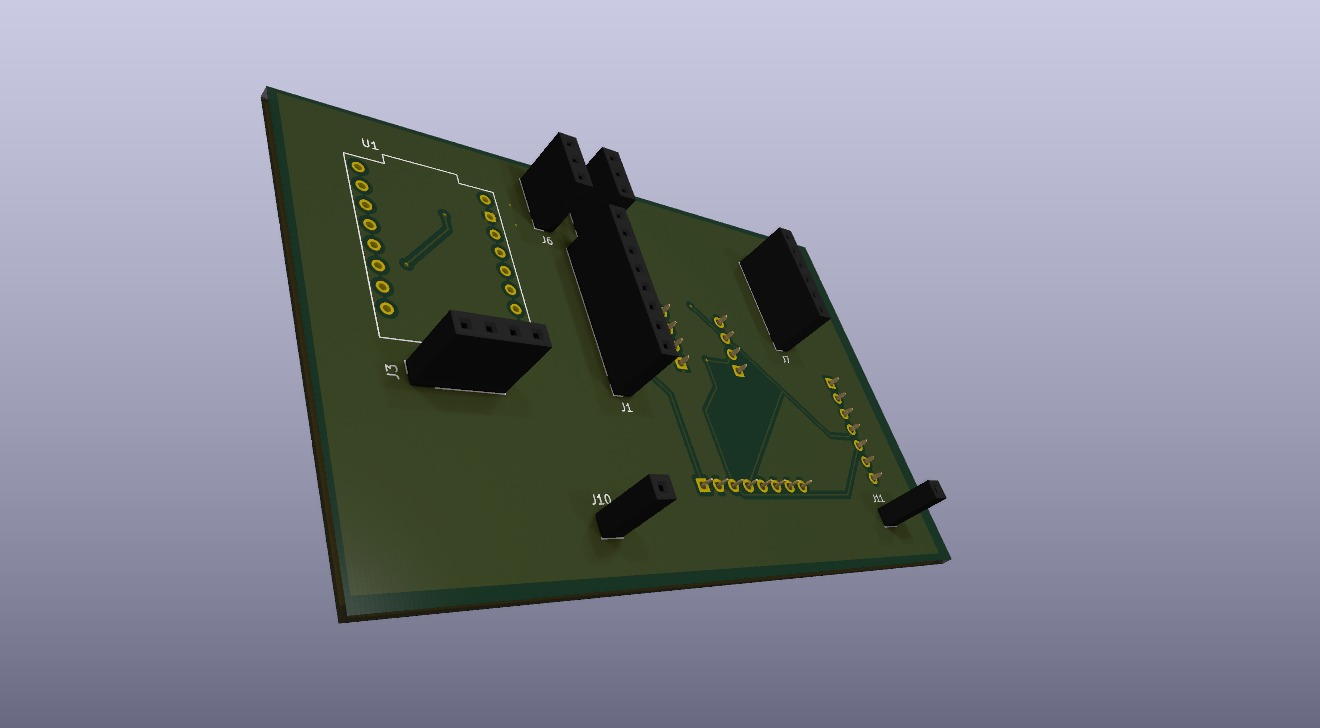
\includegraphics[width=0.48\linewidth]{foto_pcb_frontal.jpeg}
        \hfill
        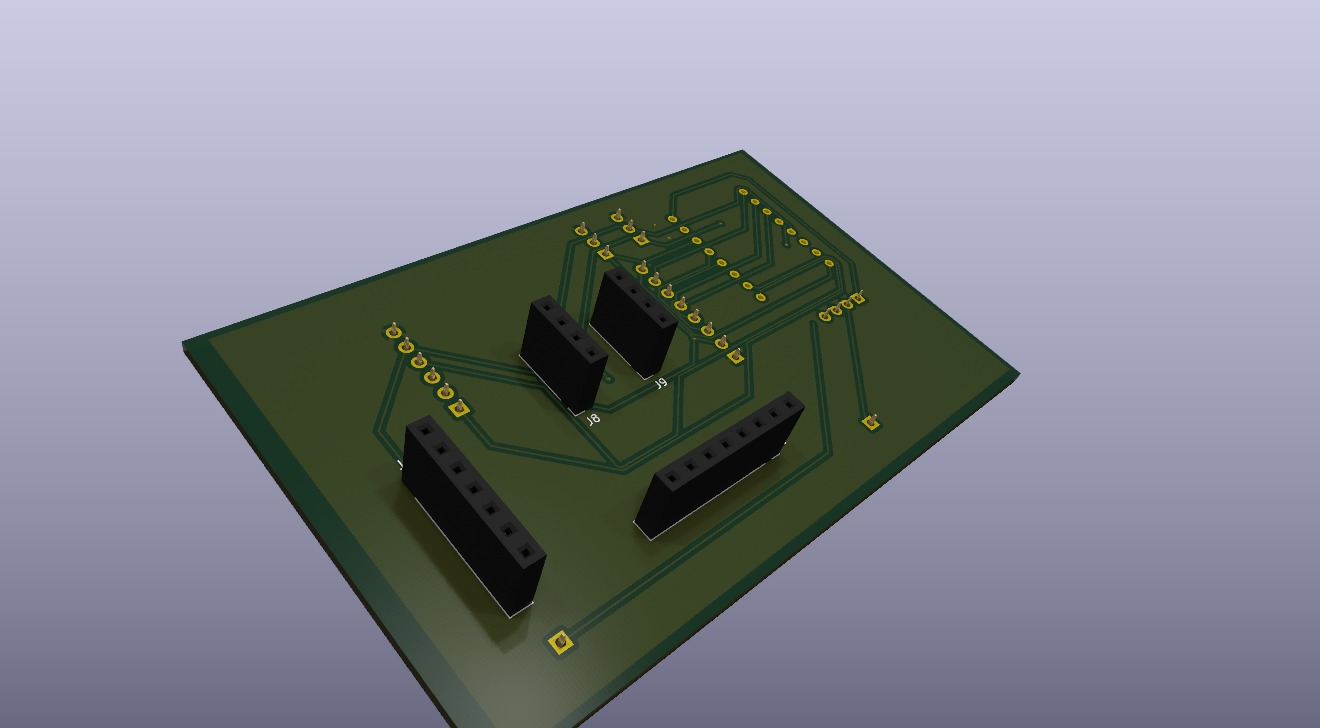
\includegraphics[width=0.48\linewidth]{foto_pcb_trasera.jpeg}
        \vspace{0.12cm}

        \scriptsize\textbf{Antes}: protoboard/perfboard para validar sensores y firmware.
        \column{0.50\textwidth}
        \footnotesize
        \textbf{Ahora}
        \begin{itemize}\itemsep0.12cm
            \item Las interfaces ya est\'an formalizadas en esquem\'atico y PCB.
            \item Se elimina incertidumbre de cableado manual.
            \item El dise\~no permite probar interferencias reales de montaje: sensor-piel, caja, botones, display y BLE.
            \item La siguiente validaci\'on relevante es de \textbf{unidad cerrada}, no s\'olo de subsistema.
        \end{itemize}
        \vspace{0.15cm}
        \begin{alertblock}{Salto de madurez}
            \scriptsize El prototipo pasa de demostrar ``que funciona'' a demostrar ``que se puede ensamblar y repetir''.
        \end{alertblock}
    \end{columns}
\end{frame}

\section{Carcasa SCAD}

\begin{frame}{Dise\~no de carcasa en OpenSCAD}
    \begin{columns}[T]
        \column{0.48\textwidth}
        \footnotesize
        \textbf{Criterios mec\'anicos}
        \begin{itemize}\itemsep0.12cm
            \item Dos mitades impresas en PLA.
            \item Ventana superior para display ST7789.
            \item Aberturas laterales para botones y USB-C.
            \item Lugs para correa intercambiable.
            \item Bottom con ventanas para PPG, temperatura y contactos ECG.
        \end{itemize}
        \vspace{0.15cm}
        \begin{block}{Ventaja de SCAD}
            \scriptsize Las cotas relevantes quedan parametrizadas: dimensiones, radios, lugs, cutouts, altura de caja y ubicaci\'on de elementos.
        \end{block}
        \column{0.52\textwidth}
        \centering
        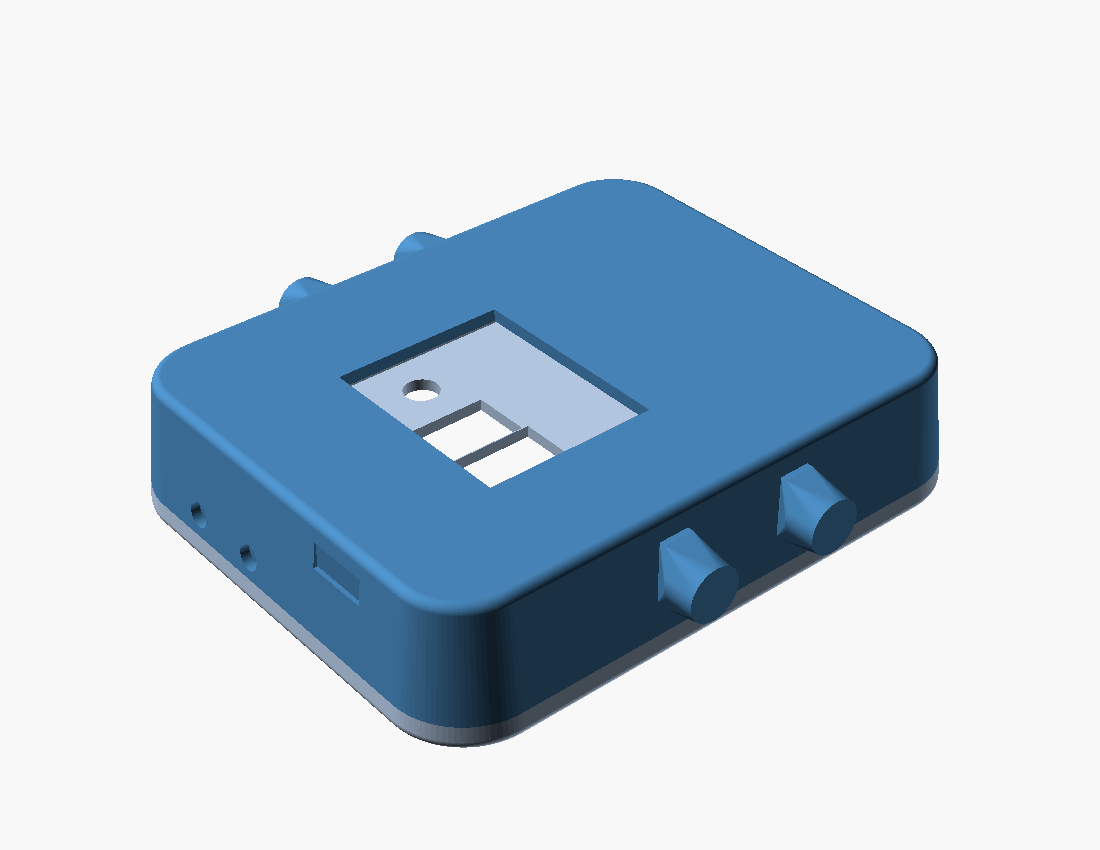
\includegraphics[width=0.96\linewidth]{render_v2_assembly_hero.png}
        \vspace{0.05cm}\newline
        \scriptsize\textbf{Figura}: Ensamble conceptual generado desde los archivos SCAD.
    \end{columns}
\end{frame}

\begin{frame}{Carcasa: vistas de integraci\'on}
    \begin{columns}[T]
        \column{0.33\textwidth}
        \centering
        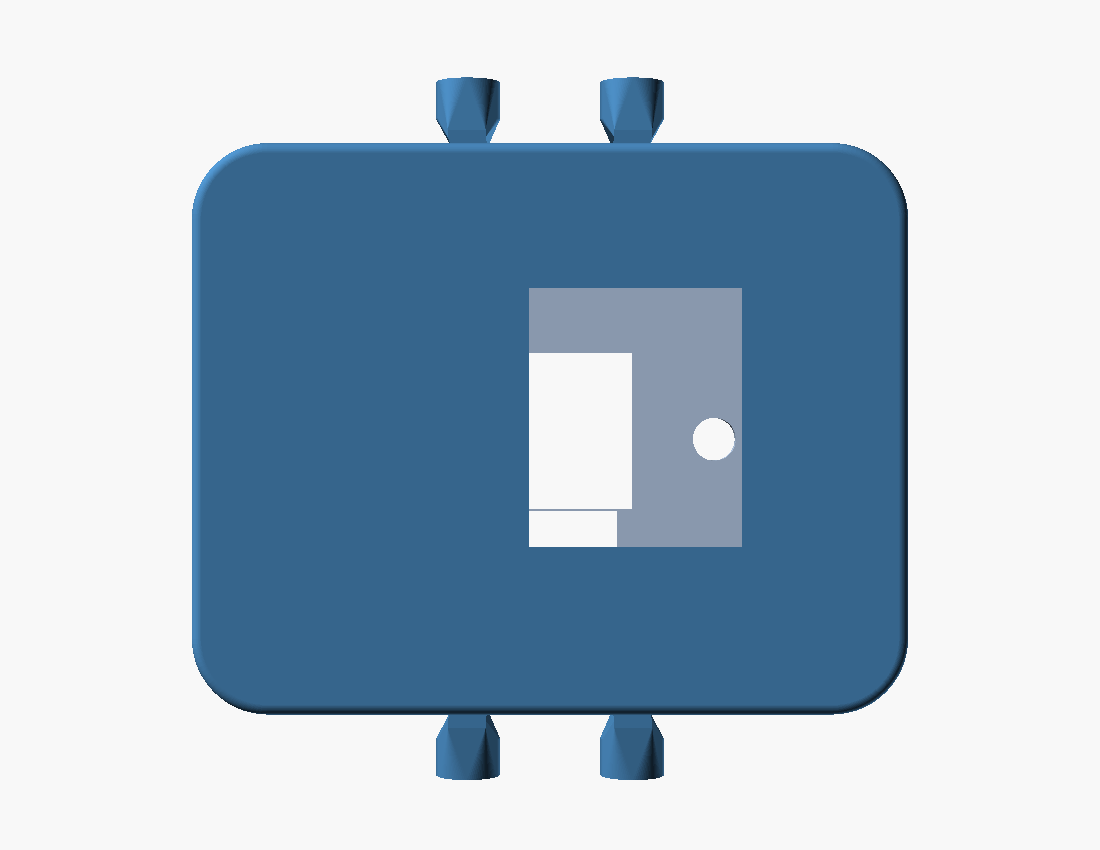
\includegraphics[width=\linewidth]{render_v2_assembly_top.png}
        \scriptsize Vista superior
        \column{0.33\textwidth}
        \centering
        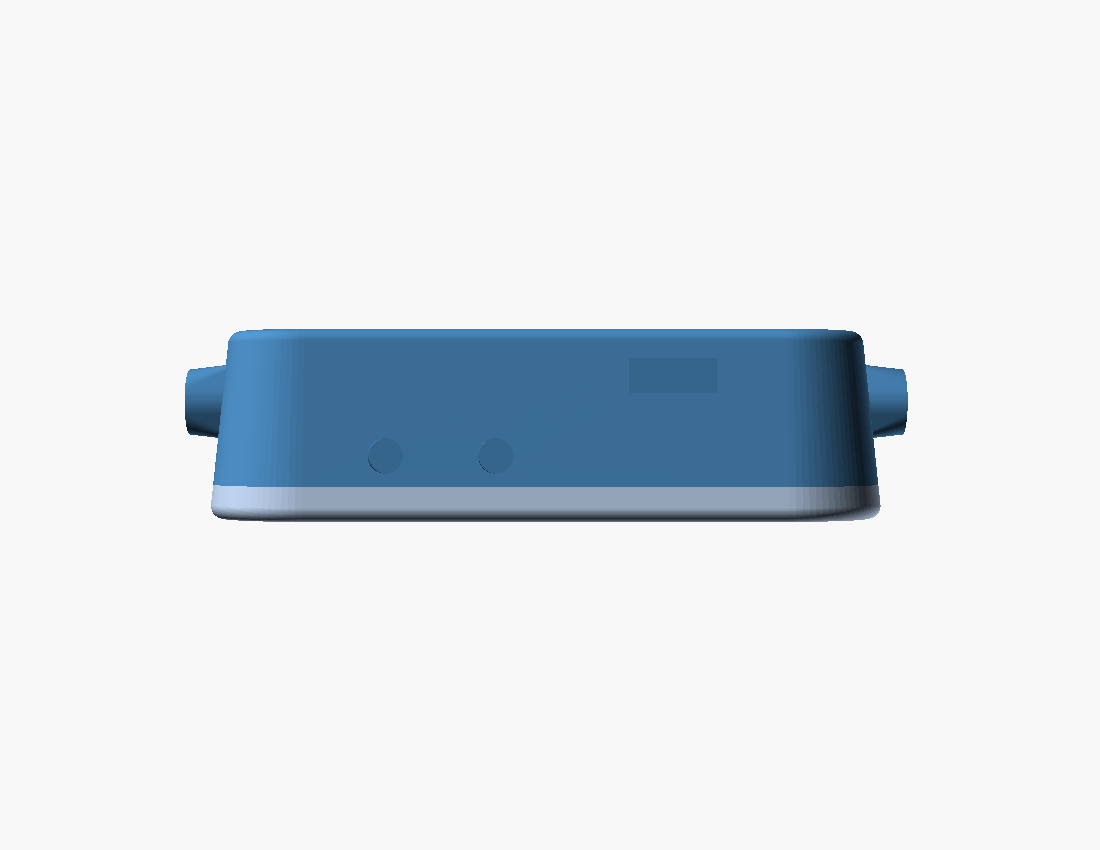
\includegraphics[width=\linewidth]{render_v2_assembly_side.png}
        \scriptsize Perfil lateral
        \column{0.33\textwidth}
        \centering
        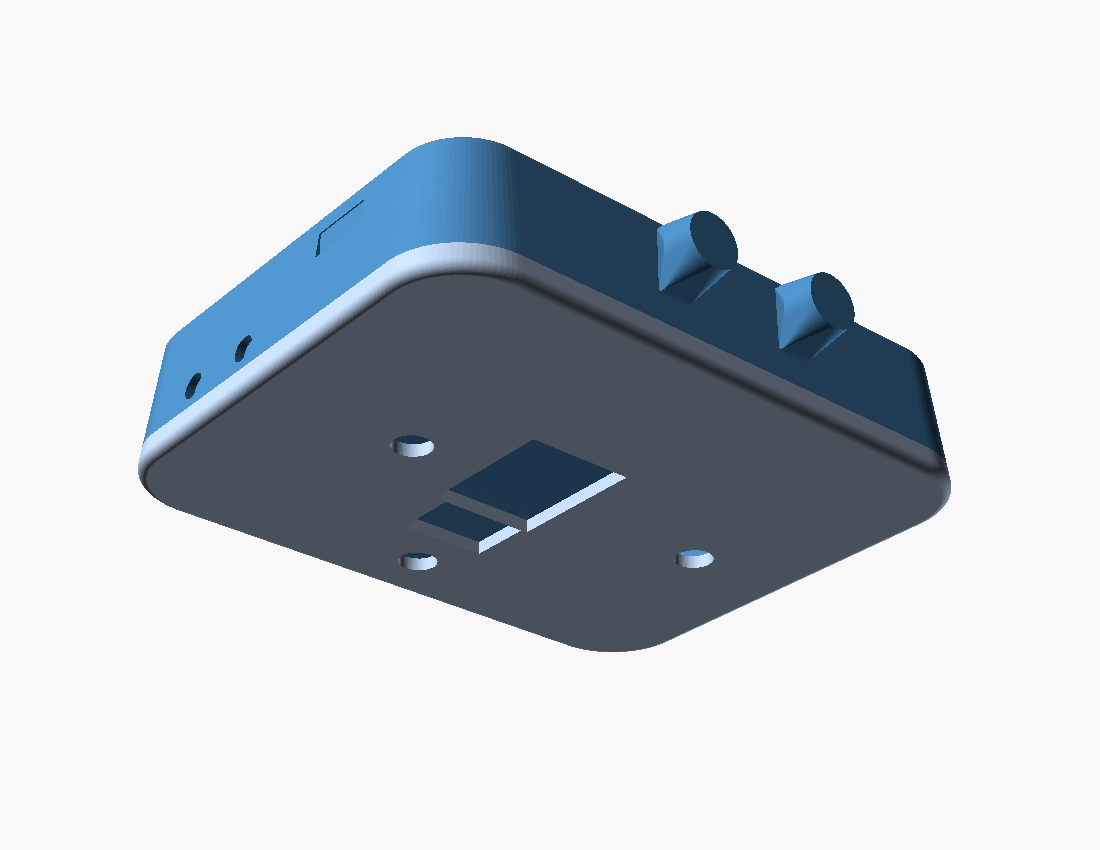
\includegraphics[width=\linewidth]{render_v2_assembly_bottom.png}
        \scriptsize Contacto con piel
    \end{columns}
    \vspace{0.25cm}
    \footnotesize
    El dise\~no mec\'anico resuelve tres interfaces cr\'iticas: alineaci\'on del display, contacto estable de sensores con piel y posibilidad de abrir/cerrar el prototipo sin destruir la PCB.
\end{frame}

\begin{frame}{Detalles mec\'anicos cr\'iticos}
    \begin{columns}[T]
        \column{0.55\textwidth}
        \footnotesize
        \begin{itemize}\itemsep0.13cm
            \item \textbf{MAX30102}: cutout circular para no bloquear el encapsulado \'optico.
            \item \textbf{MAX30205}: placa de aluminio + pad t\'ermico para mejorar acople piel-sensor.
            \item \textbf{ECG}: pernos M3 de acero inoxidable como electrodos, conectados a pads mediante pogo pins.
            \item \textbf{PCB}: standoffs y tornillos para fijar sin cargar los pads.
            \item \textbf{USB-C}: ranura lateral alineada con el conector del XIAO S3.
        \end{itemize}
        \column{0.45\textwidth}
        \centering
        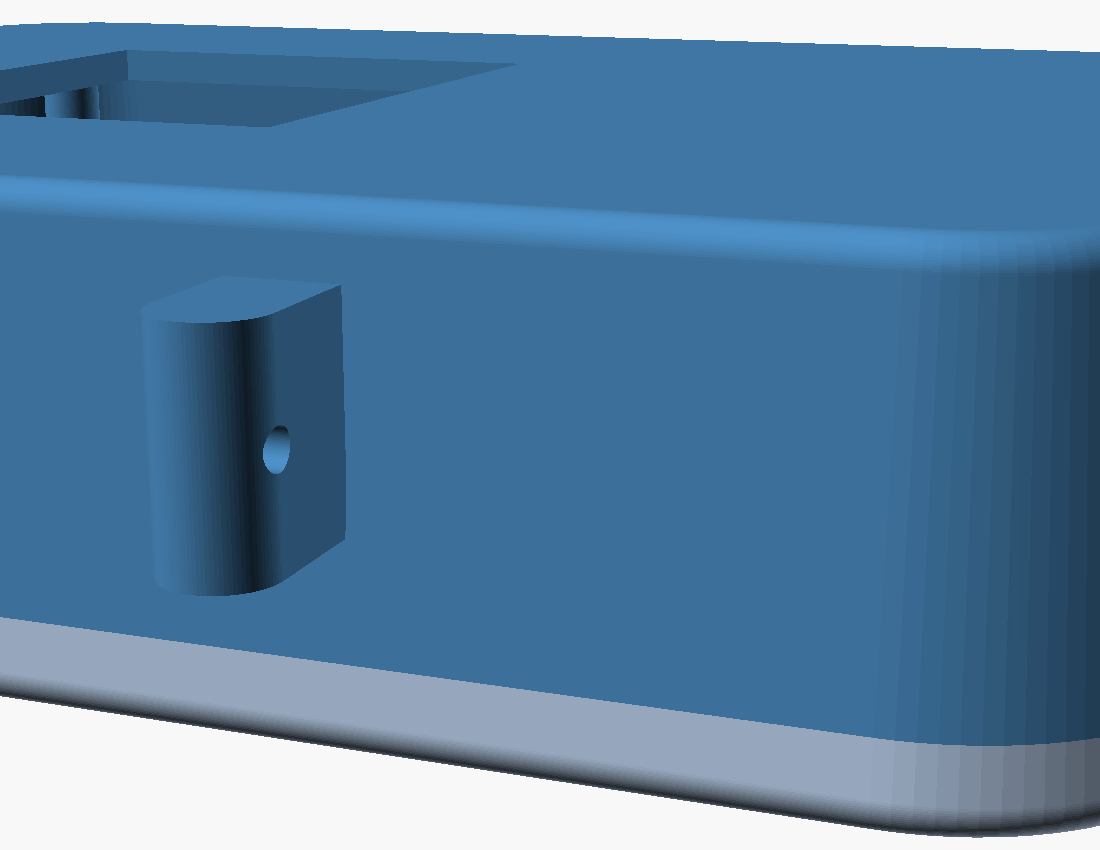
\includegraphics[width=0.78\linewidth]{render_v2_lug_closeup.png}
        \vspace{0.1cm}\newline
        \scriptsize\textbf{Figura}: Detalle de lugs y geometr\'ia de brazalete.
        \vspace{0.15cm}
        \begin{block}{Resultado}
            \scriptsize La carcasa ya no es s\'olo envolvente: participa en la calidad de medici\'on biom\'etrica.
        \end{block}
    \end{columns}
\end{frame}

\section{Pruebas}

\begin{frame}{Plan de validaci\'on de la unidad integrada}
    \footnotesize
    \begin{columns}[T]
        \column{0.48\textwidth}
        \textbf{Mec\'anica}
        \begin{itemize}\itemsep0.1cm
            \item Encaje y cierre repetido de carcasa.
            \item Alineaci\'on de botones, display y USB-C.
            \item Presi\'on estable sobre sensor t\'ermico y ventana PPG.
            \item Prueba de comodidad y peso en uso real.
        \end{itemize}
        \vspace{0.15cm}
        \textbf{El\'ectrica}
        \begin{itemize}\itemsep0.1cm
            \item Continuidad y aislaci\'on de electrodos ECG.
            \item Validaci\'on de rails 3.3 V y consumo por modo.
            \item BLE con caja cerrada.
        \end{itemize}
        \column{0.52\textwidth}
        \textbf{Funcional}
        \begin{itemize}\itemsep0.1cm
            \item HR/SpO\textsubscript{2} contra referencia externa.
            \item ECG con pernos/pogo pins vs captura directa.
            \item Temperatura con offset de carcasa caracterizado.
            \item IMU para podometr\'ia y dataset HAR.
            \item Autonom\'ia por curva del MAX17048.
        \end{itemize}
        \vspace{0.2cm}
        \begin{alertblock}{Criterio de avance}
            \scriptsize La unidad integrada debe reproducir los resultados de protoboard con degradaci\'on controlada y medible.
        \end{alertblock}
    \end{columns}
\end{frame}

\begin{frame}{Pr\'oximos pasos}
    \begin{columns}[T]
        \column{0.52\textwidth}
        \scriptsize
        \textbf{Prototipo funcional}
        \begin{enumerate}\itemsep0.08cm
            \item Limpiar el dise\~no del prototipo hasta dejarlo completamente funcional y alineado con requisitos.
            \item Cerrar DRC/ERC del carrier y validar rails, encendido y consumo en la unidad ensamblada.
            \item Repetir bring-up por subsistema con la ESP32-S3 montada en la proto.
        \end{enumerate}
        \column{0.48\textwidth}
        \scriptsize
        \textbf{ML y producto final}
        \begin{enumerate}\itemsep0.08cm
            \item Seguir tomando muestras para el modelo de Machine Learning.
            \item Avanzar a dos placas para reducir el espacio horizontal del reloj, aceptando el trade-off de mayor altura.
            \item Migrar a componentes SMD los sensores que sean m\'as f\'aciles de independizar de sus m\'odulos comerciales.
        \end{enumerate}
        \vspace{0.2cm}
        \begin{block}{Meta de la siguiente iteraci\'on}
            \scriptsize Prototipo wearable cerrado: captura biom\'etrica, visualizaci\'on local y telemetr\'ia BLE desde el carrier XIAO S3.
        \end{block}
    \end{columns}
\end{frame}

\begin{frame}[plain]
    \centering
    \vspace{1.25cm}
    {\Huge \color{main} \textbf{Demostraci\'on / Discusi\'on}}\\[0.6cm]
    {\Large XIAO ESP32-S3 + PCB carrier + carcasa SCAD}\\[0.4cm]
    \footnotesize
    Ruta de bring-up \textbar{} puntos de riesgo \textbar{} fabricaci\'on \textbar{} pruebas de unidad integrada
\end{frame}

\end{document}
